\subsubsection{Aufgabe der Komponente}
Die Broadcast Komponente ermöglicht es den Benutzern von SharkNet, Nachrichten an andere Benutzer zu schicken. Dabei können auch andere Komponenten, wie etwa der semantische Eingans- und Ausgangsfilter zum Einsatz kommen, was jedoch nicht zwingend erforderlich ist. Falls auf einen Eingangsfilter oder Ausgangsfilter verzichtet werden sollte, werden wie bei einem klassischen Broadcast die Nachrichten an alle sich in der Nähe befindlichen Geräte versendet. Inwiefern der klassische Broadcast vom Benutzer semantisch eingeschränkt werden kann, lässt sich in der Komponentenbeschreibung der Komponente Semantischer Filter in Erfahrung bringen.

\subsubsection{Architektur}

Die Komponente bildet sich vorrangig aus sieben Klassen, wovon drei sich innerhalb des SharkFrameworks und vier sich innerhalb der App befinden. Diese sieben Klassen werden nun ausgehend von der folgenden Abbildung kurz beschrieben.
\begin{figure}[H]
	\centering
	\hspace*{1cm}
	\makebox[\linewidth][c]{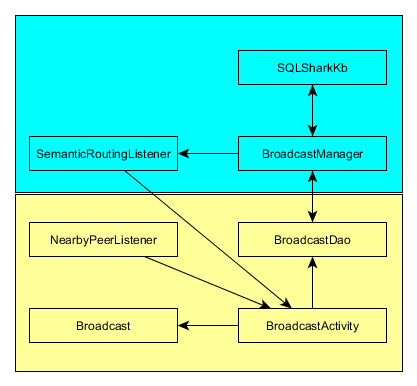
\includegraphics[width=0.6\linewidth]{general/BroadcastStruktur1.png}}%
	\caption{Die Klassen der Broadcast Komponente}
	\label{fig:broadcastStructure}
\end{figure}
\begin{itemize}
	\item Die SQLSharkKb ist eine Implementierung der Shark Knowledgebase mit SQLite. Mit ihr werden sämtliche Daten wie beispielsweise die Nachrichten, semantische Annotationen oder auch Benutzerprofile gespeichert. Sie nimmt ausschließlich Anfragen von Klassen aus dem SharkFramework entgegen.
	\item Der BroadcastManager ist die direkte Schnittstelle zwischen dem Framework und der App. Er nimmt Broadcast-Objekte vom BroadcastDao entgegen und lässt diese gegebenfalls von der SQLSharkKb speichern. Sollte eine neue Nachricht den Peer erreichen, wird vom BroadcastManager die Nachricht auf ihre semantische Relevanz hin überprüft und im Erfolgsfall der Wissenbasis des Peers hinzugefügt.
	\item Der SemanticRoutingListener liefert neue vom BroadcastManager akzeptierte Nachrichten an die BroadcastActivity
	\item Das BroadcastDao nimmt von der BroadcastActivity veränderte Nachrichten in Form eines Objekts vom Typ Broadcast entgegen, baut diese in für das SharkFramework vewertbare Objekte vom Typ ASIPSpace um und leitet diese an den BroadcastManager weiter.
	\item Wann immer die Anzahl der sich in Reichweite befindlichen Peers ändert, wird die BroadcastActivity vom NearbyPeerListener mit einer angepassten Liste von Peers versorgt.
	\item Die BroadcastActivity ist die Schnittstelle zwischen Benutzer und App. Sie nimmt neue Nachrichten vom Benutzer entgegen, wobei das Hinzufügen von semantischen Annotationen optional ist. Sie benutzt die Entitätsklasse Broadcast um die Nachrichten in einer Klasse zu bündeln, welche bei Aktualisierungen an das BroadcastDao weitergereicht werden. 
\end{itemize}


\subsubsection{Nutzung}
Die Komponente ist in der App innerhalb der \textit{BroadcastActivity} eingebunden. Der Endanwender kann über die diese Activity Nachrichten versenden, betrachten und mit semantischen Annotationen versehen, wobei Letzteres auch die Komponente Semantische Filter betrifft.
\\Die Komponente kann aber auch in eigenen Activities benutzt werden ohne die vorgegebene \textit{BroadcastActivity} benutzen zu müssen. Der Entwickler muss bei seiner eigenen Activity dafür lediglich von der Klasse \textit{BaseActivity} erben. Die Klasse \textit{BaseActivity} stellt das Attribut \textit{mApi} vom Typ \textit{SharkNetApi} bereit, mit dem durch die Methoden \textit{getBroadcast()} und \textit{updateBoradcast(...)} der Broadcast geliefert und verändert werden kann.
\\

\subsubsection{Code}
Der Code dieser Komponente kann unter \url{https://github.com/SharedKnowledge/SharkNet/tree/master/app/src/main/java/net/sharksystem/sharknet} betrachtet werden. 
\\Die Broadcast-Komponente wird vom Shark-Framework per Listener über neue Nachrichten in Kenntnis gesetzt. Der folgende Codeauszug beinhaltet die Verwertung dieser Nachrichten durch die \textit{BroadcastActivity}. \newline
 \lstset{language=Java, caption=Anzeige und Weiterleitungen von Nachrichten (Auszug), label=DescriptiveLabel, numbers=left, numbersep=1em, breaklines=true, basicstyle=\small}
\begin{lstlisting}
if (accepted) {
  broadcast = mApi.getBroadcast();
  runOnUiThread(new Runnable() {
    @Override
    public void run() {
      if(broadcast!=null){
        mAdapter.setMessages(broadcast.getMessages());
        mRecyclerView.scrollToPosition(mAdapter.getItemCount() - 1);
      }
    }
  });
  if (forwarded) {
    mApi.getSharkEngine().getBroadcastManager().sendBroadcastMessage(component, nearbyPeers);
  }
}
else {
Toast.makeText(getApplicationContext(), "Incoming Message rejected!",Toast.LENGTH_LONG).show();
}
\end{lstlisting}
Über die Parameter \textit{accepted} (Zeile 1) und \textit{forwarded} (Zeile 12) wird der \textit{BroadcastActivity} durch die vorgelagerte Filterung mitgeteilt, ob die Nachricht der Wissensbasis hinzugefügt worden ist und ob diese an andere Peers weitergeleitet werden soll. Falls die Nachricht der Wissensbasis hinzugefügt worden ist, wird die Nachrichtenliste des Broadcasts aus der Wissensbasis ausgelesen (Zeile 2) und innerhalb der Oberfläche angezeigt (Zeilen 7-8). Sollte die Nachricht neben dem Eingangsfilter auch den Ausgangsfilter passiert haben, wird die Nachricht an alle Peers in der Nähe weitergeleitet (Zeile 13). 

\subsubsection{Gerätetest}
Innerhalb der Broadcast-Komponente werden ausschließlich Oberflächenelemente genutzt, die von allen Android-Versionen (ab 4.2) genutzt werden können. Im Rahmen dieser Arbeit ist die Broadcast-Komponente abhängig von den Komponenten WiFi-Direct, Bluetooth und Radar, da sonst keine Nachrichten erfolgreich versandt und empfangen werden können. Aktuell können daher nur die Geräte den Broadcast nutzen, die zu den drei Komponenten kompatibel sind.
\begin{table}[H]
	\begin{center}
		\caption{Kompatibilitätstests im Überblick}
		\label{tab:testsAll}
		\begin{tabular}{l|c|c|c|c|c} 			
			Gerät & Version & WiFi-Direct & Bluetooth & Radar & Broadcast \\
			\hline
			LG Nexus 5x & 8.0 & Ja & Ja & Ja & Ja\\
			LG Nexus 5x & 8.1 & Ja & Nein & Ja & Nein\\
			LG Nexus 5 & 6.1 & Ja & Ja & Ja & Ja\\
			Sony Xperia XZ Premium & 8.0 & Ja & Ja & Ja & Ja\\
			Sony Xperia Z4 Tablet & 7.1.1 & Ja & Ja & Ja & Ja\\
			Lenovo B & 6.0 & Ja & Ja & Ja & Ja\\
			Lenovo A5500-F Tablet & 4.4 & Nein & Nein & Ja & Nein\\
			Raspberry Pi 3 & 6.0.1 & Nein & Ja & Ja & Nein\\	
			Wandboard Quad & 5.0.2 & Nein & Ja & Ja & Nein\\			
		\end{tabular}
	\end{center}
\end{table}
\subsubsection{Ausblick}
Der Austausch von Nachrichten mit mehreren Geräten in der Nähe funktioniert grundlegend sicher, aber noch nicht komplett fehlerlos. So kann es bei hoher Last seitens der Benutzer passieren, dass einige Nachrichten nicht empfangen werden können, obwohl sie gemäß dem eingestellten semantischen Filter akzeptiert werden müssten. 
\newpage